\chapter{Resultados} % Main chapter title
\label{Chapter3 } % For referencing the chapter elsewhere, use 

\section{Nivel educativo}

Para el caso del nivel educativo, es importante conocer la cantidad de alumnos por año en cada nivel, de esta forma identificamos si existe algún incremento o alguna disminución, para lo que se deberá realizar diversas acciones contrarrestando cualquier inconveniente de materiales y de inmobiliarios. Ver la imagen~\ref{fig:niveleseducativos}

\begin{figure}[h]
\centering
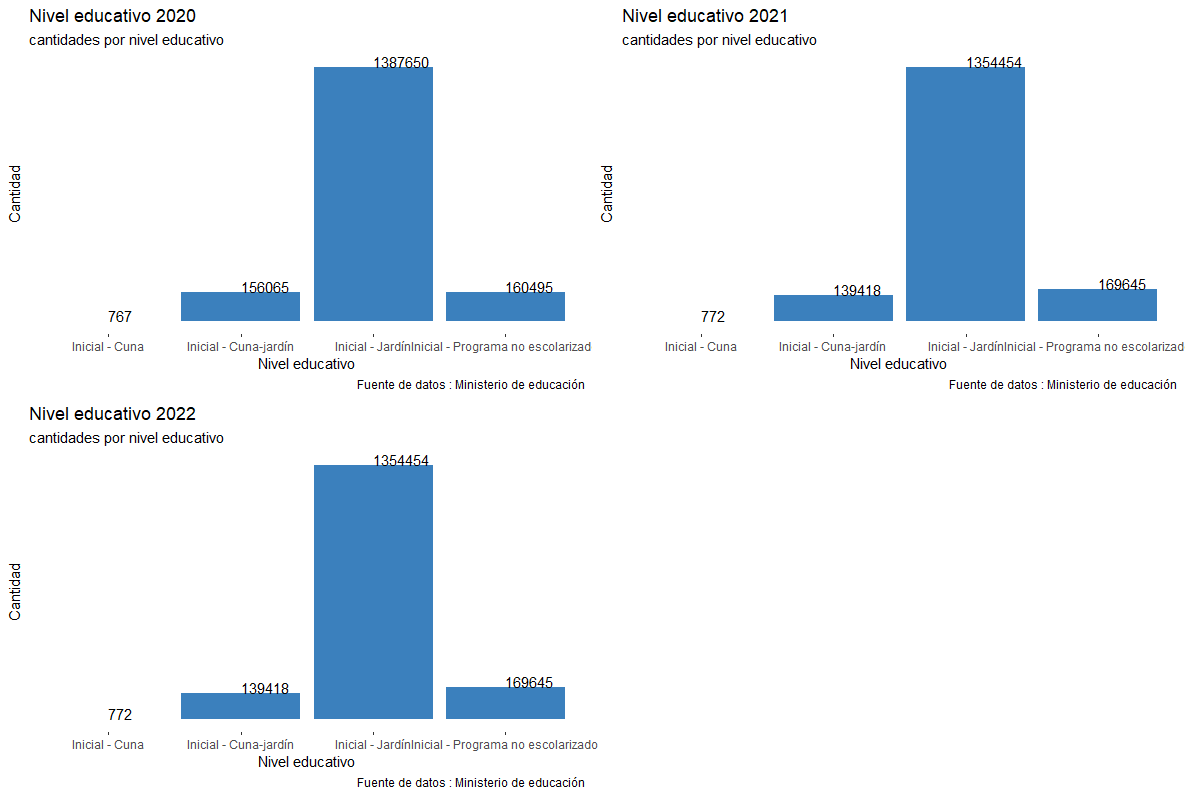
\includegraphics[width=1.2\textwidth]{Figures/nivelesEducativos}
\decoRule
\caption[Nivel Educativo]{Niveles educativos}
\label{fig:niveleseducativos}
\end{figure}

\section{Evolución mensual de matrículas}\label{res_evolucion_matriculas}

En este análisis se identificó la evolución que han tenido la cantidad de matrículas de cada mes en los últimos 3 años, las siguientes imágenes~\ref{fig:matriculas} muestran la evolución por año.\\
Se aprecia una mayor cantidad de incidencias entre Marzo y Abril, esto se puede entender por el inicio del año escolar en el Perú. Y en menor medida hay una cantidad elevada de matrículas desde el inicio de año, durante el resto del año se ve una menor cantidad pero si ocurren, esto podría deberse posiblemente a traslados de colegio.

\begin{figure}[h]
\centering
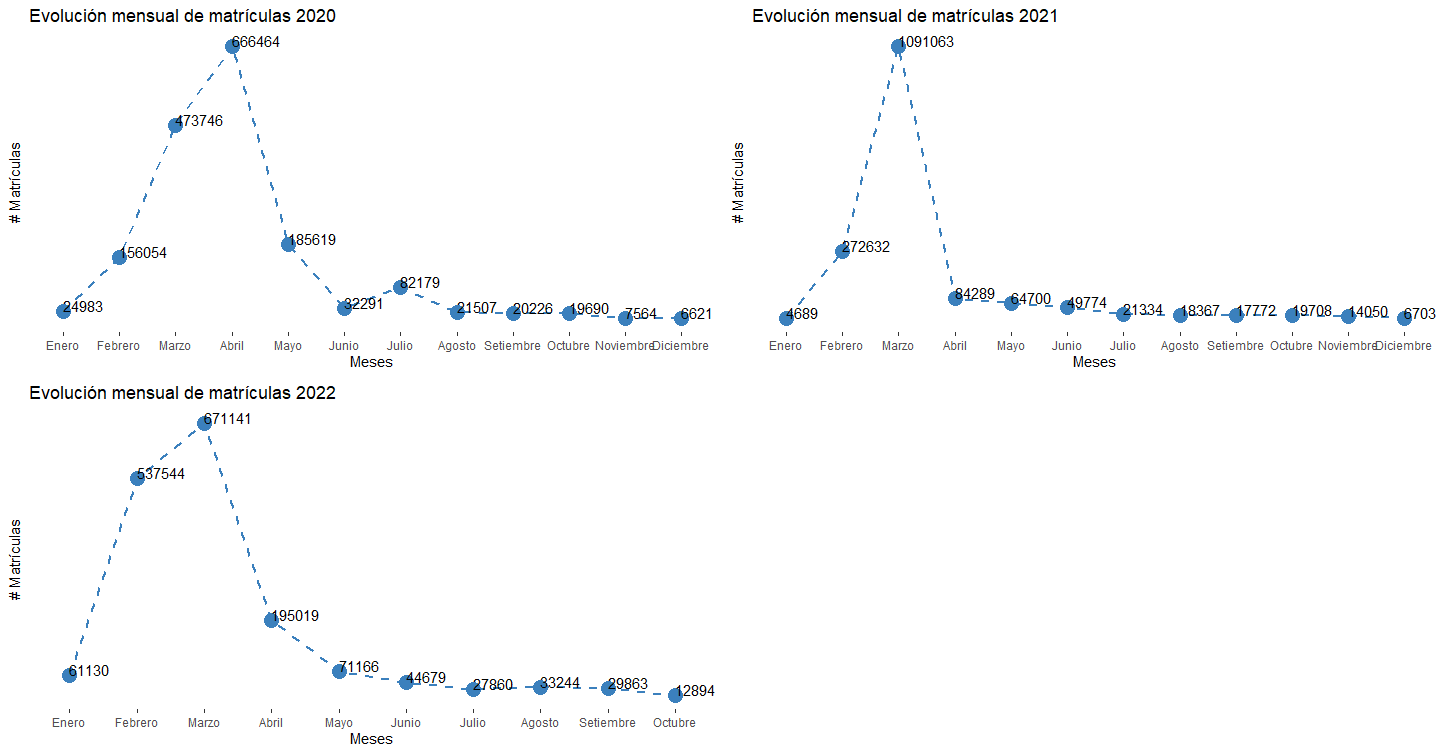
\includegraphics[width=1.2\textwidth]{Figures/evolucionMatriculas}
\decoRule
\caption[Matrículas]{Evolución de cantidades por cada mes}
\label{fig:matriculas}
\end{figure}

\section{Discapacidad}

El presente gráfico~\ref{fig:discapacidad} queremos mostrar la cantidad de estudiantes con alguna discapacidad sea visual, sordoceguera, autismo, auditiva entre otros.\\
Se puede apreciar que en los últimos 2 años se tenía mayor incidencia en las discapacidades motora, intelectual y autismo, pero en el presente año han disminuído las que tienen que ver con motora e intelectual, pero el autismo se mantiene como un factor predominante.

\begin{figure}[th]
\centering
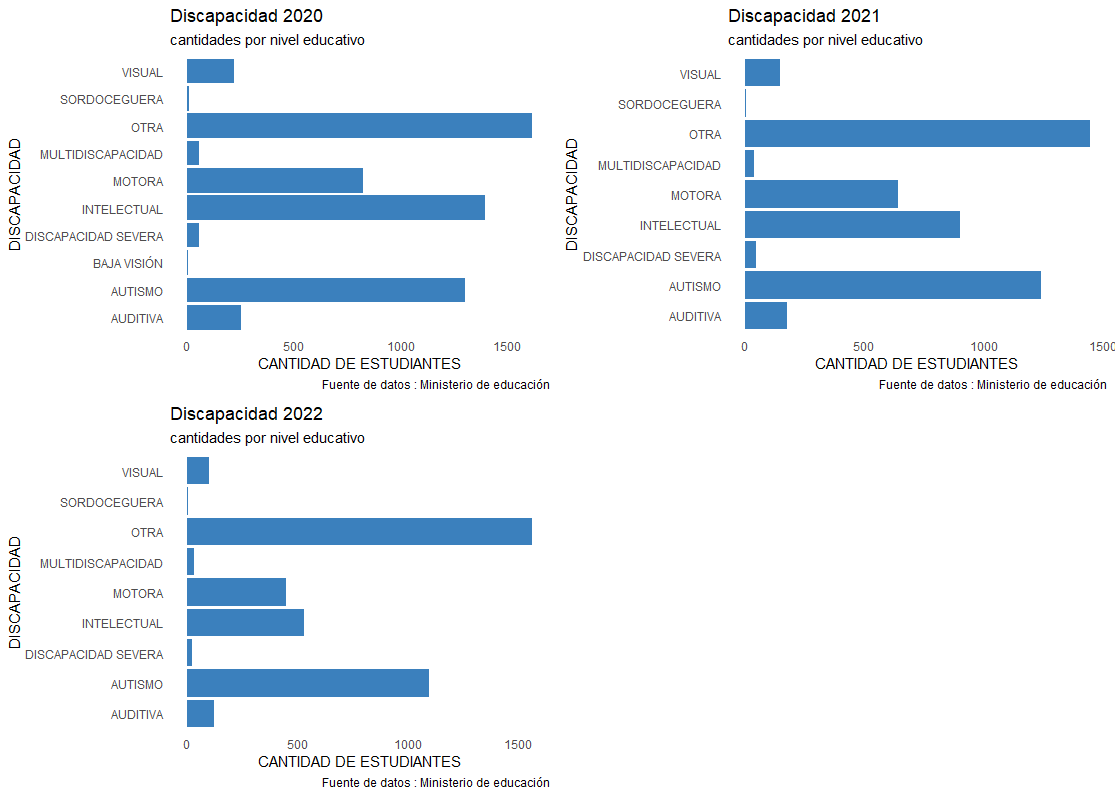
\includegraphics[width=0.8\textwidth]{Figures/discapacidad}
\decoRule
\caption[Discapacidad]{Tipos de discapacidad}
\label{fig:discapacidad}
\end{figure}


\section{Nacionalidad de estudiantes}

Se muestra a continuación una imagen~\ref{fig:nacionalidad} la distribución de nacionalidades, teniendo como mayor cantidad, luego de la peruana, la nacionalidad Venezolana, debido a que hay muchos países en este análisis, se ve conveniente el uso de una tabla para poder mostrar los datos.

\begin{figure}[!h]
\centering
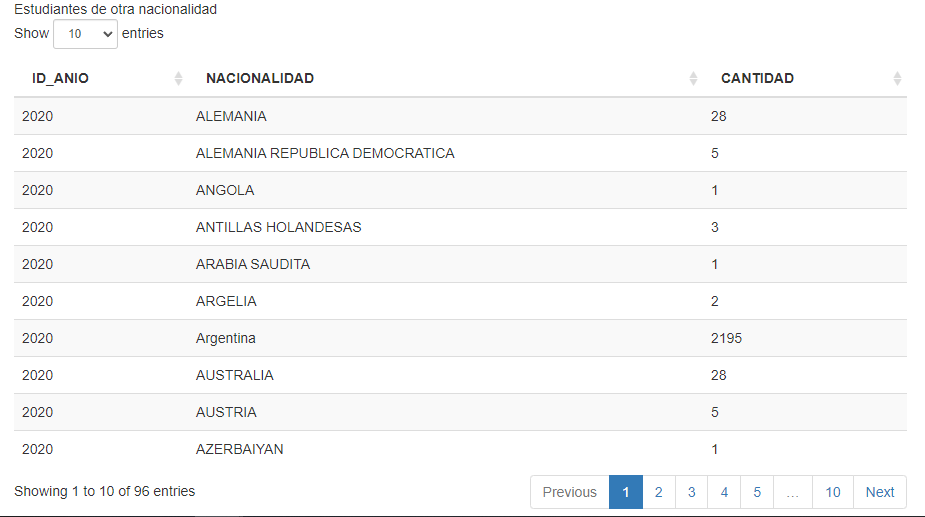
\includegraphics[width=1\textwidth]{Figures/nacionalidad}
\decoRule
\caption[Nacionalidad]{Nacionalidad de estudiantes}
\label{fig:nacionalidad}
\end{figure}

\section{Distribución de género}

En la imagen~\ref{fig:genero} se pueden apreciar distribuciones simulares entre hombres y mujeres.

\begin{figure}[!h]
\centering
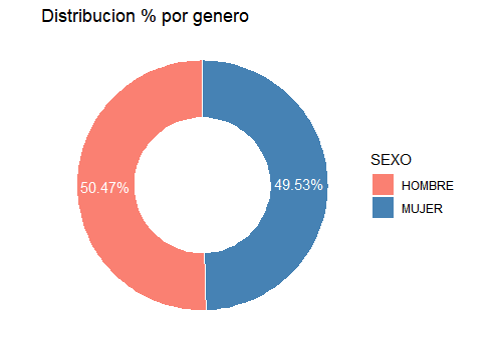
\includegraphics[width=0.8\textwidth]{Figures/genero}
\decoRule
\caption[Genero]{Distribuciones de género}
\label{fig:genero}
\end{figure}

\section{DNI Validados}

En la imagen~\ref{fig:validaciondni} se aprecia que hay una gran mayoría de documentos validados, pero se ve en menor medida estudiantes indocumentados.

\begin{figure}[!h]
\centering
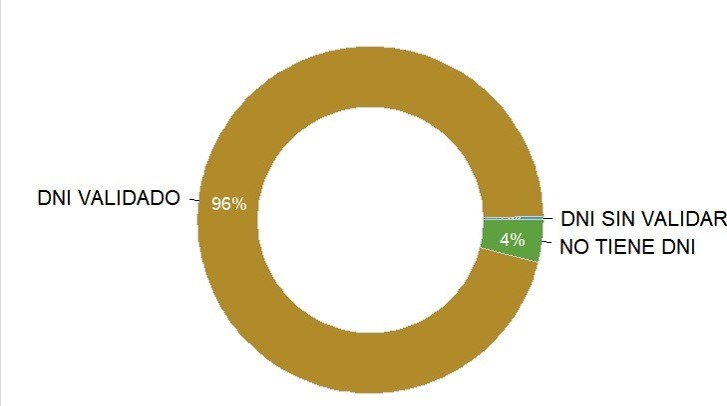
\includegraphics[width=0.8\textwidth]{Figures/validacionDNI}
\decoRule
\caption[DNI Validados]{Validaciones de DNI}
\label{fig:validaciondni}
\end{figure}

\section{Representación por Shiny}
En shiny se desarrolló un panel que tiene un filtro por año para poder filtrar los gráficos presentados anteriormente según la imagen~\ref{fig:shiny}, la reactividad ante este campo de entrada permite tener la visualización de lo que ocurre por año.
\begin{figure}[th]
\centering
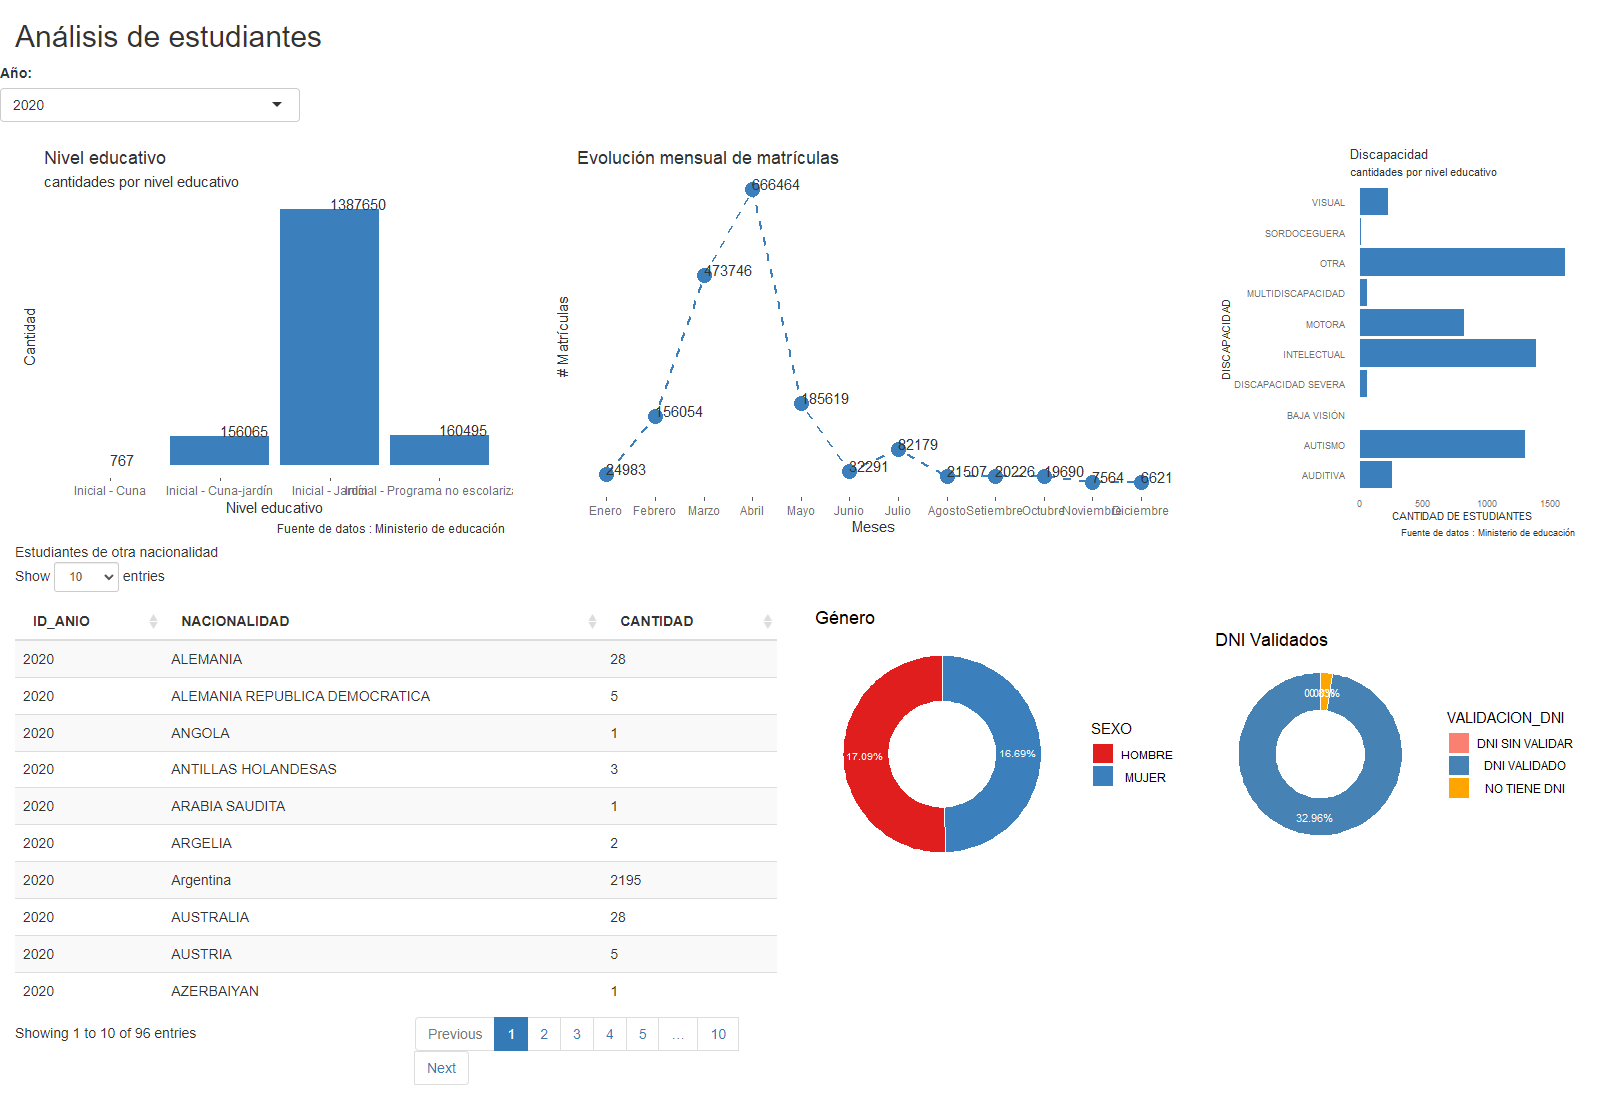
\includegraphics[width=1\textwidth]{Figures/shiny}
\decoRule
\caption[Shiny]{Representación mediante Shiny}
\label{fig:shiny}
\end{figure}

\section{Representaciones de ubicación de instituciones educativas por mapa}

Ya que es importante conocer la ubicación de los colegios, se realizó un mapa utilizando las librerias ggplot2, tidyverse y mapview en R, esta última librería proporciona funciones para crear visualizaciones interactivas de datos espaciales de manera muy rápida y conveniente. El código de estas representaciones se encuentra en el anexo \ref{cod_mapas}

Diagrama~\ref{fig:mapa1}: Su objetivo principal es llenar el vacío del trazado interactivo rápido (sin grado de presentación) para examinar e investigar visualmente ambos aspectos de los datos espaciales, las geometrías y sus atributos

\begin{figure}[th]
\centering
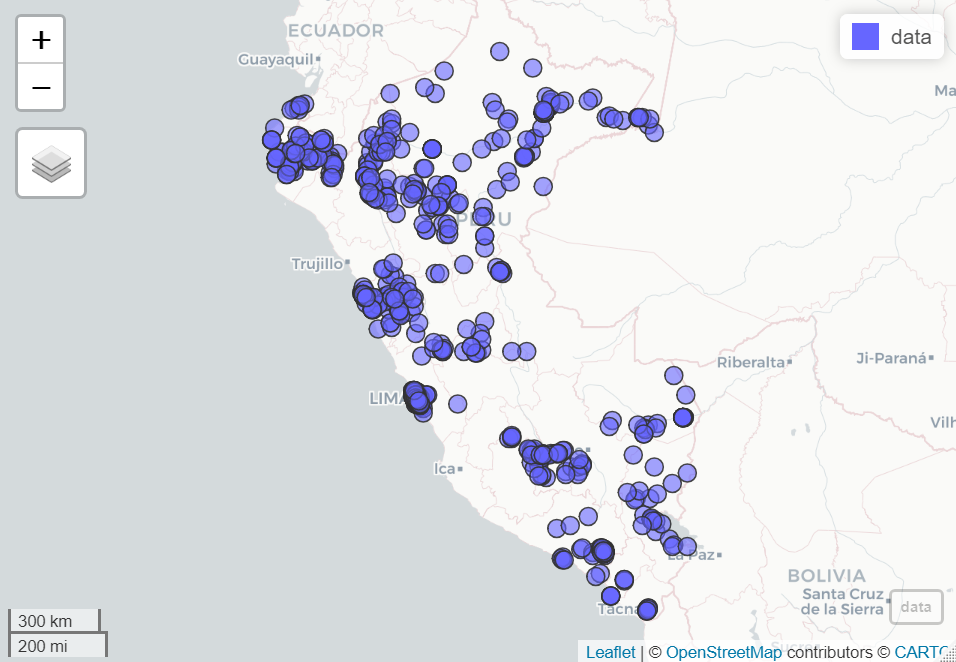
\includegraphics[width=1\textwidth]{Figures/mapa1}
\decoRule
\caption[Mapa]{Representación geográfica}
\label{fig:mapa1}
\end{figure}

Diagrama~\ref{fig:mapa2}: También podemos ver un conteo rápido del número de colegios por sector, con la librería leaflet, con una muestra que se extrajo, podemos ver a medida que vamos aumentando el zoom en que zonas entan mayor concentrados los colegios. 

\begin{figure}[th]
\centering
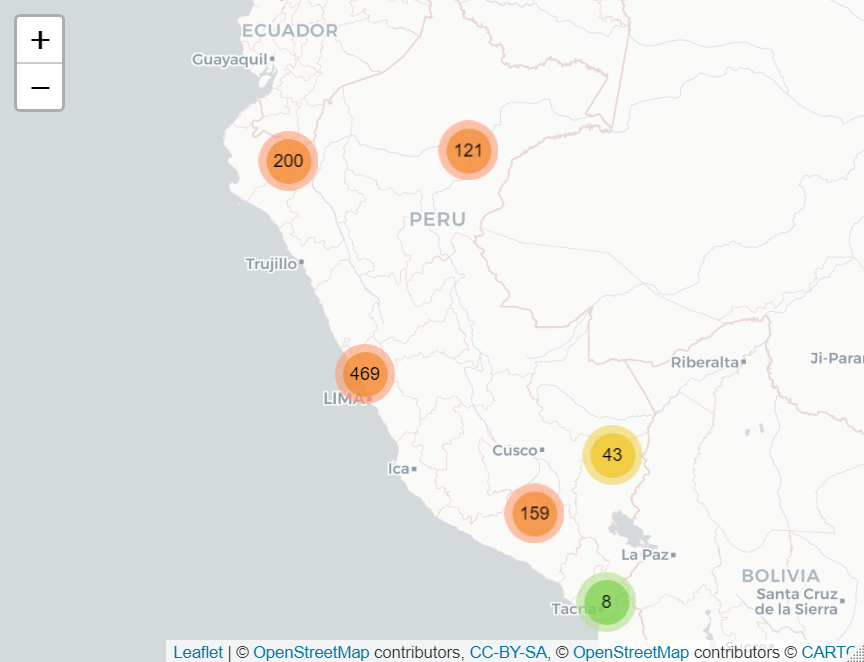
\includegraphics[width=1\textwidth]{Figures/mapa2}
\decoRule
\caption[Mapa]{Colegios}
\label{fig:mapa2}
\end{figure}

Diagrama~\ref{fig:mapa3}:Aprovechamos la interactividad del gráfico y cada que acercamos (zoom) nos muestra la cantidad de colegios acumulados en cada zona.

\begin{figure}[th]
\centering
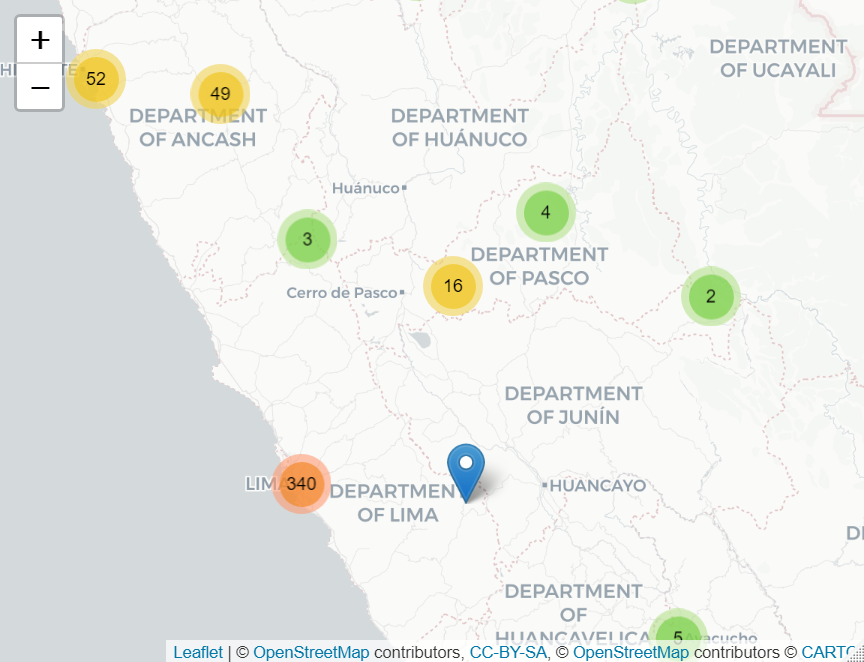
\includegraphics[width=1\textwidth]{Figures/mapa3}
\decoRule
\caption[Mapa]{Instituciones educativas acumuladas}
\label{fig:mapa3}
\end{figure}